\chapter{Diskussion: \textit{Where’s morphology?}}
\label{chap:10}
Wenngleich die Darstellung der Untersuchungsergebnisse in den vorangegangenen Kapiteln primär deskriptiv ausgerichtet war, wurden bereits einige Aspekte thematisiert, die stärker im sprachtheoretischen Rahmen der Arbeit zu verorten sind. Zentral war hier vor allem das Verhältnis von Form und Funktion. In \chapref{chap:7} bestand die methodische Schwierigkeit in der Abgrenzung, wann eine innerparadigmatische Alternation rein phonologisch bedingt ist und wann sie genuin morphologisch ist, d.\,h. funktionalisiert und evtl. sogar produktiv. Eine (zumindest vorläufige) Lösung dieses methodischen Problems war die Einbeziehung der mentalen Repräsentation: Gibt es überhaupt Alternationen, die rein phonologisch bedingt sind und die für die Sprecher/Hörer keinerlei morphologische Information symbolisieren? Sämtliche Alternationen wurden daher grundsätzlich im Phänomenbereich der Morphologie verortet und aus der Perspektive morphologischer Kodierung beschrieben. Inwiefern diese Lösung auch außerhalb der spezifischen Herausforderungen der Datenklassifikation tragfähig und plausibel mit Blick auf die kognitive Verankerung von Pluralmarkern ist, ist unter anderem Thema des folgenden Kapitels.

Die empirischen Befunde werden dabei nicht noch einmal im Detail dargestellt, sondern sie werden gebündelt und unter Einbeziehung von morphologischer Theoriebildung diskutiert. Die Diskussion knüpft dabei an die Leitfrage von Teil~\ref{part:II} an: „Where’s morphology?“ Grundlegend ist wieder das Verständnis von Flexion als grammatischem Schnittstellenphänomen, das heißt, nicht nur das isolierte Wort, sondern auch der morphosyntaktische und semantisch-pragmatische Kontext werden in die Überlegungen einbezogen. Im Einzelnen geht es um folgende Aspekte:

\begin{itemize}
\item In welchem Verhältnis stehen Form und Funktion, und zwar in den rezenten Flexionssystemen sowie diachron in der Entwicklung der Deklinationsklassen?
\item Wo ist Flexionsmorphologie im mentalen Lexikon zu verorten?
\item Inwiefern ist Flexionsmorphologie an andere Systemebenen gekoppelt?
\item Wie können Variabilität in der formalen Realisierung und fakultative Markierung in einem Grammatikmodell berücksichtigt werden?
\end{itemize}

\begin{sloppypar}
Ziel ist es, die dialektalen Flexionssysteme vor dem Hintergrund der theoretischen Ansätze zu vergleichen und durch die Anwendung der morphologischen Theorien auf dialektale Daten gleichzeitig deren Validität und explanatives Potenzial zu überprüfen. Die Diskussion bezieht sich dabei auf die in \chapref{chap:5} vorgestellten Modelle: \sectref{sec:10.1} fokussiert die Form-Funktions-Ebene aus Perspektive der Natürlichen Theorie, in \sectref{sec:10.2} wird dieser Aspekt vor dem Hintergrund der Vorhersagen des Relevanzprinzips diskutiert. \sectref{sec:10.3} und damit das gebrauchsbasierte Schema-Modell nach \citet{Köpcke1993} bilden schließlich Abschluss und Schwerpunkt des Kapitels.
\end{sloppypar}

\section[head=Natürliche Morphologie]{Natürliche Morphologie: Flexion zwischen optimaler Kodierung und Redundanz}
\label{sec:10.1}
Die Voraussage der Natürlichen Morphologie ist, dass sich (unter der Prämisse von Morphologie als geschlossenem, autonomen System) optimale morphologische Kodierungen herausbilden. Optimale Kodierungen sind nach \citet[22]{Mayerthaler1981} „konstruktionell ikonisch, uniform und transparent“, das heißt, sie entsprechen dem Prinzip „one function -- one form“ und ein semantisches „Mehr“ wird auch durch ein formales „Mehr“ ausgedrückt (ausführlicher \sectref{sec:5.1}). Die dialektalen Flexionssysteme des Oobd. unterlaufen dieses Ideal optimaler morphologischer Kodierungen, indem es ausgeprägte Allomorphie und eine Tendenz zu kumulativer Markierung gibt (die beide das Ideal „one function -- one form“ unterlaufen). Gleichzeitig widersprechen der hohe relative Anteil von rein stammaffizierenden Markierungen und Nullpluralen dem Ideal der konstruktionellen Ikonizität, die graduell beschrieben wird.  \figref{fig:18} zeigt exemplarisch für das nordbair. Nabburg, dass die untersuchten Dialekte das gesamte Spektrum von maximal und minimal ikonischen bis hin zu nicht- und kontra-ikonischen Kodierungen abdecken (in Form innerparadigmatischer Konsonantismusalternationen des Typs K/0).


\begin{figure}%10.1
\begin{tikzpicture}\footnotesize
		\matrix (hierarchy)
		[matrix of nodes, 
		nodes in empty cells,
		nodes={text width=2.8cm, align=center},
		row sep=.2cm
		]
		{
			& & & \\[0.1ex]
			maximal ikonsch & minimal ikonisch & nicht-ikonisch & kontra-ikonisch \\
			b{\aufstrichOgonek}ǫu – b{\aufstrichOgonek}ǫum ,Bub` & v\=iš – viʃ̌ ,Fisch` & hēvα – hēvα ,Hafen` & lōαb – l\^{ǫ}i ,Laib`\\
			biəkɑ – biəkɑn ,Birke` & haud – hait ,Haut` & ạntn̥ – ạntn̥ ,Ente` & mōαd – mōi ,Magd`\\
		};
		\draw [left color=black, 
		right color=white]
		(hierarchy-1-1.north west) rectangle (hierarchy-1-4.south east);
	\end{tikzpicture}
\caption{\label{fig:10.1}Hierarchie des konstruktionellen Ikonismus (Beispiele aus dem nordbair. Nabburg)}
\label{fig:18}
\end{figure}

In Teilen kann dieser Befund durch lautgesetzlichen Wandel erklärt werden, daneben spiegelt die Formenbildung der rezenten Dialekte das Ineinandergreifen phonologischer und morphologischer Prozesse wider. Durch die Apokope des Schwa-Suffixes entfällt in den Dialekten des UGs zunächst ein maximal ikonisches Verfahren. Die „Störungen“ \citep[43]{Mayerthaler1981} des konstruktionellen Ikonismus, die die Phonologie hier verursacht hat, werden gleichzeitig durch lautgesetzlichen, d.\,h. ebenfalls phonologischen Wandel kompensiert und zum Teil von der Morphologie funktionalisiert: Durch Einsilberdehnung, den Diph"-thong"-wech"-sel bei mhd. \textit{ei} und mittelbair. Konsonantenschwächung entstehen lautgesetzlich innerparadigmatische Kontraste der Vokalquantität, -qualität und des Konsonantismus und damit minimal ikonische Kodierungen, die zumindest eingeschränkt produktiv sind (vgl. \citealt[98]{Harnisch2016}, \citealt[43--44]{Rowley1997}). Im Falle von Subtraktion und K/0-Alternationen führen Lenisierungen sogar zu kon"-tra-""i"-ko"-ni"-schen Symbolisierungen. Die Frage ist nun: Warum halten sich diese weniger als maximal ikonischen Symbolisierungen seit Jahrhunderten weitestgehend im Paradigma? Und inwiefern sind rein stammaffizierende Markierungen tatsächlich weniger optimale Kodierungen einer morphologischen Kategorie?

\begin{sloppypar}
Eine Lösung dieser Fragen findet sich in späteren Arbeiten zur Natürlichen Morphologie, die die Prinzipien der Natürlichen Morphologie und sprachökonomischen Ansätze integrieren (ausführlicher \sectref{sec:5.1}). \citet{Harnisch1988} etwa ergänzt das Streben nach optimaler Kodierung um „kognitionsökonomische“ Prinzipien. Die lexikalische Speicherung von irregulären oder suppletiven Flexionsformen ist kognitiv vorteilhaft und ökonomischer, da auf tokenfrequente Formen schneller zugegriffen werden kann. Morphologische Irregularität ist gleichzeitig ein „Differenzierungsverfahren“ \citep[185]{Nübling2004}, da der Erhalt irregulärer Flexionsformen Synkretismen im Flexionsparadigma und damit nicht-ikonische Kodierungen verhindert. Nicht-segmentierbare, d.\,h. minimal ikonische oder kontra-ikonische Markierungen, symbolisieren die morphologische Information damit per se nicht schlechter, sondern nur anders (siehe auch \citealt{BybeeNewman1995} und \citealt[379]{Harnisch2000}).
\end{sloppypar}

Herausgefordert werden die Vorhersagen der Natürlichen Morphologie da, wo die Morphologie zu „Störungen“ des konstruktionellen Ikonismus und zur Aufhebung morphologischer Distinktionen führt: durch die Generalisierung des Nasalsuffixes im Paradigma der Feminina des Typs \teuthoo{das\#n}{dašn} -- \teuthoo{das\#n}{dašn} ‚Tasche‘, die auf innerparadigmatischen, morphologischen Ausgleich zurückgeht. Und auch die kumulativen (und damit nicht-optimalen) Markierungen in \teuthoo{s\#du.2m}{šdūͅm} -- \teuthoo{ds\#di"mA}{dšdīmα} ‚Stube‘ und \teuthoo{o4<b5v5l°@}{ộb̩v̩l̥̑} -- \teuthoo{epfl°@n@}{epf‌l̥̑n̥} ‚Apfel‘ (nordbair.-mittelbair. Bernhardswald) sind nicht das Ergebnis phonologischer Prozesse, sondern sekundärer morphologischer Markierungen (vgl. \sectref{sec:8.3.3.1}).

Dass kumulative Markierungen durch Morphologie geschaffen werden, kann das Konzept der Systemangemessenheit nach \citet{Wurzel1984} erklären. Im südlichen Nordbair. wird eine additive Pluralmarkierung mit Nasal- oder Tiefschwa-Suffix durch eine prosodische Input-Konditionierung bei Maskulina und Feminina auf Reduktionssilbe mhd. -\textit{el}, -\textit{en}, -\textit{er} gefordert. Im Tiefenbohrungspunkt Bernhardswald tritt die Suffigierung auch an Stämme, die bereits Umlautplural aufweisen: Pl. \teuthoo{ds\#di"mA}{dšdīmα} ‚Stuben‘, \teuthoo{ds\#na\$wl°@n@}{dšna̤wl̥̑n̥} ‚Schnäbel‘, \teuthoo{epfl°@n@}{epf‌l̥̑n̥} ‚Äpfel‘. Hier wäre die fehlende Suffigierung nicht systemangemessen, auch wenn dies zu einer redundanten, kumulativen Markierung der Pluralinformation führt (vgl. \citealt[99]{Harnisch2016}, \citealt[43]{Rowley1997}).

\begin{sloppypar}
Während minimal und kontra-ikonische Formen genauso wie kumulative Markierungen durch die Berücksichtigung von Systemangemessenheit und Ge"-brauchs"-fre"-quenz mit den (erweiterten) Annahmen der Natürlichen Morphologie durchaus in Einklang gebracht werden können, bleibt die Frage: Wie wird der hohe Anteil von Nullpluralen insbesondere bei den Feminina im nördlichen Nordbair. und im Ofr. erklärt? Die morphologische Kategorie wird hier auch nicht durch den Artikel kodiert, da Formensynkretismus vorliegt (\teuthoo{di}{di} \teuthoo{das\#n}{dašn} -- \teuthoo{di}{di} \teuthoo{das\#n}{dašn}). Während sich in einem Teil des Bair. eine ikonische, additive Markierung des Typs \teuthoo{das\#nA}{dašnα} herausgebildet hat, die sogar auf einige Maskulina analogisch übertragen wird (\textit{boumα} ‚Buben‘, \textit{okßnα} ‚Ochsen‘, vgl. \citealt[149]{Wildfeuer2001}), halten sich im Ofr. die fem. Nullplurale. Der Dialektvergleich zeigt zum einen, dass die Dialektsysteme unterschiedliche Strategien entwickelt haben, um mit ähnlichen (durch die Morphologie verursachten) Voraussetzungen umzugehen. Dass Teile der untersuchten Dialekte die Numerussynkretismen nicht abgebaut haben, weist darauf hin, dass diese die Stabilität des Flexionssystems nicht gefährden (vgl. \citealt[181]{HarnischRowley1990}, \citealt[145]{Mauser1998a}, \citealt[200]{Rowley1997}). Die nicht-ikonische Symbolisierung der Pluralinformation scheint hier den Status eines normalen und systemangemessenen Strukturmerkmals zu haben.
\end{sloppypar}

\section{Relevanzprinzip: Numerusprofilierung und Kasusnivellierung}
\label{sec:10.2}
Die Vorhersage des Relevanzprinzips nach \citet{Bybee1985b} lautet, dass
(1) der Relevanzgrad einer Kategorie und der Grad an Fusionierung zwischen zwei Einheiten korrelieren,
(2) dass die Reihenfolge der lexikalischen oder flexivischen Ausdrücke am Stamm durch Relevanz gesteuert ist und
(3) dass relevante Kategorien diachron stabiler sind (siehe \sectref{sec:5.2}). Die fortschreitende Numerusprofilierung und gleichzeitige Nivellierung des Kasusausdrucks als zentrale Tendenzen nominalmorphologischen Wandels im Deutschen kann also durch unterschiedliche Relevanzgrade der beiden Flexionskategorien erklärt werden. Und auch die Entwicklungen in den untersuchten Dialekten zeigen, dass Numerus relevanter ist als Kasus. Doch lohnt hier der Blick ins Detail, da sich erst dort zeigt, dass die dialektalen Entwicklungen in Teilen auch eine Herausforderung für die Vorhersagen des Relevanzprinzips darstellen.

Der hohe Anteil fusionierender Ausdrücke, der durch die große Vielfalt stammaffizierender Verfahren und durch analoge Umlautplurale in den Daten zu finden ist, weist Numerus als eine hochrelevante Kategorie aus. Zudem sind die dialektalen Flexionssysteme durch ein hohes Maß an Allomorphie geprägt, was ebenfalls auf die Relevanz einer Kategorie hinweist (vgl.
\citealt{DammelNübling2006}). Auch der höhere kognitive Aufwand, der mit der ganzheitlichen Speicherung von lexikalisierten morphophonologischen Alternationen verbunden ist (etwa im Falle der arbiträren, „ablautähnlichen“ Vokalwechsel im Nordbair.), deutet auf die Relevanz von Numerus hin. Dass innerparadigmatische Vokalquantitäts- und Lenis-Fortis-Kontraste, die lautgesetzlich im Plural und zudem im Dat.Sg. entstanden waren, konsequent im Bereich der Kasus-, nicht aber in der Numeruskodierung abgebaut wurden, weist auch in diese Richtung (siehe \sectref{sec:7.2.1}, vgl. \citealt[63--65]{Birkenes2014}).

Generell ist eine Tendenz zum Abbau der Kasusflexion am Substantiv zu beobachten, teilweise besteht sogar eine Tendenz zu Kasussynkretismen in der Nominalphrase (\sectref{sec:9.1}). Eine formale Kodierung der Kasusflexion ist im Singular nur in den obliquen Kasus der schwachen Maskulina und im Bair. bei den Verwandtschaftsbezeichnungen erhalten (vgl. \sectref{sec:7.2.2}). Im Pluralparadigma findet sich eine distinkte Dativ-Plural-Form vor allem im Nordbair. und im Oberofr.: \teuthoo{vi"EglAn}{vīəɡlαn} ‚Vögel‘
(nordbair. Tirschenreuth), \teuthoo{den}{den} \teuthoo{glan}{ɡlan} \teuthoo{ma2dlana}{mādlana} ‚den kleinen Mädchen‘ (ofr. Hallerstein, vgl. \mapref{map:24}). Bemerkenswert ist einerseits, dass sich hier teilweise sogar Allomorphie herausgebildet hat, deren Distribution teilweise frei, teilweise phonotaktisch und im nördlichen Nordbair. durch eine präferierte Outputstruktur gesteuert ist. Andererseits wurde in \sectref{sec:9.1.2} gezeigt, dass das Auftreten der distinkten Dativ-Plural-Form vor allem auch durch den morphosyntaktischen Kontext bedingt ist: In Präpositionalphrasen mit pluralischer NP wird die flexivische Information präferiert am Substantiv kodiert, während der Artikel reduziert wird oder entfällt: \teuthoo{in}{in} \teuthoo{a4rmAn}{ạrmαn} ‚in den Armen‘ (nordbair. Tirschenreuth), \teuthoo{a4m}{ạm} \teuthoo{ne4s5dnAn}{nẹs̩dnαn} \teuthoo{dra.n}{draͅn} ‚an den Ästen dran‘ (nordbair.-mittelbair. Blaibach). Aus Perspektive des Relevanzprinzips stellt sich die Frage, welche die relevante Information ist, die am Substantiv kodiert wird. Sämtliche Fälle formaler (teilweise fakultativer) Dativ-Plural-Markierung, die in \sectref{sec:9.1.2} diskutiert wurden, deuten darauf hin, dass es die Pluralinformation und damit die relevante Numeruskategorie ist, die hier dis\-ambiguiert wird (siehe auch \sectref{sec:7.2.2}).

Auch die fakultativen Markierungen, die in einem Teil des Bair. bei den \textit{n}{}-erweiterten Feminina funktionalisiert sind, dienen der Disambiguierung der Pluralinformation (siehe \sectref{sec:9.2}). Wenn der morphosyntaktische oder se\-man\-tisch-prag\-ma\-ti\-sche Kontext die Numerusinformation nicht disambiguiert, wird der Numerussynkretismus morphologisch durch einen flexivischen Ausdruck am Substantiv aufgefangen: \teuthoo{na4<e4<e4}{nậệệ} \teuthoo{glo4<k,nA}{ɡlộk͓nα} ‚neue Glocken‘ -- \teuthoo{mi."4}{mị̄ͅ} \teuthoo{de}{de} \teuthoo{ga.<nt,S,n@}{ɡâͅnt͓ʃ͓n̥} \teuthoo{glo4<k,n@}{ɡlộk͓n̥} \teuthoo{la4<e4<d5n@}{lậệd̩n̥} ‚mit den ganzen Glocken läuten‘ (mittelbair. Reischach). Dass sich hier eine Art Hintertür entwickelt hat, um den vollständigen Abbau des Numerusausdrucks zu vermeiden, zeugt wiederum von der Relevanz der Numeruskategorie. In diesem Sinne lassen sich auch die „Doppelsuffigierungen“ bei den Feminina mit \textit{n}{}-Erweiterung einordnen, die im südlichen Nordbair. und in Teilen des Mittelbair. in allen Gebrauchskontexten erscheinen (\mapref{map:29}). Hier hat sich systematisch eine morphologische Strategie herausgebildet, um die Pluralinformation formal am Substantiv zu kodieren und distinkte Singular- und Pluralformen zu schaffen.

Dass dies aber nur in einem Teil der Dialekte geschehen ist, stellt einen großen Widerspruch zu den Vorhersagen des Relevanzprinzips dar. Der Numerussynkretismus der Feminina des Typs \teuthoo{das\#n}{dašn} -- \teuthoo{das\#n}{dašn} ‚Tasche‘ ist auch deshalb so faszinierend, weil (1) der ebenfalls synkretische Definitartikel (\textit{die} -- \textit{die}) keine Disambiguierung leistet, (2) der Synkretismus überhaupt erst durch die Morphologie (nämlich innerparadigmatischen morphologischen Ausgleich) geschaffen wurde und (3) die dialektalen Flexionssysteme -- mit Ausnahme der genannten Teile des Bair. -- den Synkretismus nicht abbauen. Die Lösung dieses Widerspruchs scheint darin zu liegen, dass kommunikative Strategien außerhalb des Phänomenbereichs der morphologischen Theoriebildung liegen und diese jene nicht in mögliche Entwicklungsszenarien morphologischer Systeme integrieren. Auch \citet{Harnisch1984} zeigt für den Genussynkretismus in der starken Adjektivflexion im ofr.-nordbair. Grenzgebiet (\teuthoo{A}{α} \teuthoo{blindA}{blindα} ‚ein(e) blinde(r)‘), dass Dialektsprecher kommunikative Strategien im Gespräch nutzen, um entstandene Formensynkretismen bei einer relevanten flexivischen Kategorie zu disambiguieren (siehe \sectref{sec:4.2.2}). Dass der Numerussynkretismus der typenfrequenten Klasse der historischen fem. \textit{n}{}-Deklination in einem großen Teil der oobd. Dialekte nicht beseitigt wurde, ist ein weiterer Beleg dafür, dass der Abbau der flexivischen Distinktion „ohne Schaden möglich war“ \citep[89]{Harnisch1984}, und dass morphologische Systeme im Hinblick auf die Deflexion relevanter Kategorien belastbarer sind, als angenommen und durch das Relevanzprinzip modelliert.

\section{Dialektale Schemata}
\label{sec:10.3}
Vor dem Hintergrund des in \sectref{sec:5.3} vorgestellten Schema-Modells werden im Folgenden die Aspekte mentale Repräsentation und Perzeption morphologischer Markierungen fokussiert. Die Grundannahme des Schema-Modells besteht darin, dass sprachliches Wissen im Lexikon in Form von prototypisch strukturierten Mustern organisiert ist und dass bei der Produktion und Perzeption auf diese abstrakten Schemata zurückgegriffen wird. Für die Perzeption ist dabei entscheidend, dass die Kategorisierung sprachlicher Einheiten (etwa als Singular- oder Pluralform) probabilistisch ist und einzelne Struktureigenschaften mehr oder weniger prototypisch für die assoziierte Funktion sind.

\citeua{Köpcke1993} analysiert die Pluralallomorphie des Deutschen mit Blick auf abstrakte Schemata, die mit den morphologischen Informationen Singular und Plural assoziiert sind (siehe \sectref{sec:5.3.2}). Basis dieser abstrakten Schemata sind „mögliche singulare und plurale Gestalten“ \citep[85]{Köpcke1993} von Substantiven, die Sprecher/Hörer des Deutschen gespeichert haben. Ausgangspunkt der Analysen sind also die konkreten Struktureigenschaften von Singular- und Pluralformen. Da sich dialektale Flexionssysteme durch ein spezifisches Markerinventar und spezifische Strukturmerkmale von Singular- und Pluralformen auszeichnen, sind hier auch andere, nämlich spezifisch dialektale Schemata und Prototypen anzunehmen. Ziel dieses Kapitels ist es, solche abstrakten Schemata für die untersuchten Dialekte vorzuschlagen.

\subsection{Dialektale Cues und spezifische Signalstärke}
\label{sec:10.3.1}
Nach \citet{Köpcke1988, Köpcke1993} basiert die probabilistische und prototypische Struktur eines Schemas auf der Signalstärke (\textit{cue strength}), die sich aus den perzeptuellen Charakteristika der einzelnen Cues des Schemas ergibt und die auf den Kriterien Salienz, Typen- und Tokenfrequenz, Validität und Ikonizität basiert (siehe hierzu \sectref{sec:5.3.3}).\footnote{Bedingt durch die Spezifik des BSA-Korpus können im Folgenden keine Aussagen über Tokenfrequenz getroffen werden; hierfür bräuchte es Datenmaterial, das nicht aus Erhebungsdaten besteht, sondern Sprachgebrauch etwa in Form von spontansprachlichem Material dokumentiert.} Als ein Befund ist hinsichtlich dieser Kriterien zunächst festzuhalten, dass dialektale Pluralmarker im Vergleich zum standarddeutschen Markerinventar weniger ikonisch sind und nicht-silbenbildende Verfahren (Stammaffizierung, Null) ausgesprochen frequent sind (siehe \sectref{sec:10.1}). Sie sind weniger salient, wenn man Salienz wie \citet[82]{Köpcke1993} auf Segmentierbarkeit und die wortfinale Position bezieht. Und auch die Validität der einzelnen Cues ist eine andere. So ist der Pluralmarker -\textit{(e)n} in den untersuchten Dialekten weniger valide als im Standard, weil er als Strukturmerkmal der Feminina mit \textit{n}{}-Erweiterung (Typ \teuthoo{das\#n}{dašn} -- \teuthoo{das\#n}{dašn} ‚Tasche‘) auch im Singular ausgesprochen typenfrequent ist. Infolge der Apokope des Schwa-Suffixes weisen die untersuchten oobd. Dialekte im Bereich der additiven Markierung zwei Suffixe auf, die zwar salient und ikonisch sind, aber jeweils eine geringe Validität als Hinweisreiz für die Pluralinformation haben: Sowohl -\textit{en} als auch -\textit{er} sind bei zahlreichen Singularstämmen zu finden.

 \tabref{fig:19} schematisiert die Merkmale, die für die abstrakten singularischen und pluralischen Schemata in den untersuchten Dialekten definierend sind, und schlägt eine Anordnung dieser Cues auf dem Kontinuum zwischen prototypischen Singular- und Plural-Schemata vor. Inwiefern diese Anordnung der tatsächlichen Signalstärke und der Position der einzelnen Cues im Verhältnis zueinander entspricht, muss indes noch empirisch überprüft werden; die Abbildung ist vielmehr eine Hypothese ausgehend von den dialektalen Flexionsstrategien und ihrer Distribution.


\begin{table}
\small
\begin{tabularx}{\textwidth}{>{\raggedright\arraybackslash}p{.2\textwidth}lQQQQQ}
\lsptoprule
& Singular &  &  &  & & Plural\\
& \tikzmark{sg} &  &  &  & & \hphantom{Plural}\tikzmark{pl}\\\midrule
Definitartikel (reduziert/Vollform) & \makecell[tl]{\textit{(ə)s} /\\\textit{des}} & \textit{dα} / \textit{deα} &  & {\textit{d}‘ / \textit{di}} & & \\
\tablevspace
Silbenanzahl &  &  & ein\-silbig & mehr\-silbig &  & \\
\tablevspace
Umlaut &  & {[$-$Umlaut]} &  &  & {[+Umlaut]} &\\
\tablevspace
Vokalquantität &  & {[$-$kurz]} &  & & {[+kurz]} &\\
\tablevspace
Lenis/Fortis & Lenis &  &  &  &  & Fortis\\
\tablevspace
stammfinaler Konsonant &  & {Elision} & & & {Erhalt} &\\
\tablevspace
Reduktionssilbe &  &  & & {ofr. \textit{{}-n}

bair. \textit{{}-n}} & \textit{{}-er}

\textit{{}-α} & {Nasal+ \textit{α /-αn}}\\
\lspbottomrule
\end{tabularx}
\caption{Schematische Darstellung der Strukturmerkmale (Cues) auf dem Kontinuum der abstrakten Singular- und Plural-Schemata nach \citet{Köpcke1993} (vgl. \citealt[212]{DomahsEtAl2017})\label{fig:19}}
\begin{tikzpicture}[overlay,remember picture,>={Triangle[]}]
\draw[<->,thick] (pic cs:sg) -- (pic cs:pl);
\end{tikzpicture}
\end{table}

Für den Hinweisgeber Definitartikel ist eine ähnliche Signalstärke wie auch im Standard anzunehmen, da sich die Distribution der Artikelformen im Casus rectus nicht unterscheidet; allerdings müssen reduzierte und Vollformen differenziert werden (siehe \sectref{sec:9.1.1}). \citet[87]{Köpcke1993} zufolge ist die Signalstärke des Definitartikels \textit{die} etwas größer für die Funktion Plural als für Singular (vgl. \citealt[224--225]{DomahsEtAl2017}). Da die Artikelform \textit{dα}/\textit{deα} nicht nur die Information des Nom.Sg. der Maskulina, sondern auch die Information des Dat.Pl. der Feminina signalisiert, ist die Validität und damit die Signalstärke des mask. Definitartikels geringer als die des neutr. Artikels \textit{(ə)s}/\textit{des}.

Bedingt durch den lautgesetzlich erfolgten Wandel der historischen \textit{i}{}- und \textit{a}{}-Deklination ist das Merkmal der Silbenanzahl insofern uneindeutig, als diese typenfrequenten Klassen in den rezenten Dialekten einsilbige (minimal und nicht-ikonische) Pluralformen aufweisen. Die Form des Pluralsuffixes der mehrsilbigen additiven Formen stellt -- wie oben bereits eingeführt -- ebenfalls kein eindeutiges Merkmal der Pluralität dar. In jenen ofr. Dialekten, die auch synchron die Suffixe mhd. -\textit{en} und -\textit{er} differenzieren, weist -\textit{er} (wie auch im Standard) eine relativ niedrige Validität auf (vgl. \citealt[84]{Köpcke1993} und \sectref{sec:5.3.2}). Das (Pseu\-do-)Suffix -\textit{en} (bzw. dessen heteromorphische Entsprechung) ist als Pluralmarker der historisch schwachen Maskulina, der wenigen schwachen Neutra und der Feminina mit apokopiertem Singularstamm zwar typenfrequent, doch ist die Validität von -\textit{en} als Hinweisgeber für die Pluralinformation infolge der Generalisierung des Nasalsuffixes im Paradigma der Feminina des Typs \teuthoo{das\#n}{dašn} -- \teuthoo{das\#n}{dašn} gering.

In den bair. Dialekten, wo die Reduktionssilben mhd. -\textit{en} und -\textit{er} synchron nicht differenziert werden und wo die Distribution der Reduktionssilben -\textit{n} und \mbox{-\textit{α}} für mhd. -\textit{en} phonologisch bedingt ist, muss eine andere Signalstärke für Tief"-schwa-""Re"-duk"-tions"-sil"-be angenommen werden. Die Reduktionssilbe -\textit{α} erscheint hier nicht nur als Pseudosuffix bei den Lexemen mit mhd. -\textit{er} (Typ \teuthoo{vensdA}{vensdα} ‚Fenster‘) und als genustypisches Pluralsuffix der Neutra, sondern auch bei Feminina und Maskulina mit Reduktionssilbe mhd. -\textit{en} (\teuthoo{biEkA}{biəkα} ‚Birke‘, \teuthoo{haofA}{haofα} ‚Haufen‘). Als Folge der „Doppelsuffigierung“ der Feminina und teilweise der Maskulina mit Reduktionssilbe -\textit{n}/-\textit{α} durch Tiefschwa- respektive Nasal-Suffix (Typ \teuthoo{das\#nA}{dašnα} und \teuthoo{haofAn}{haofαn}) erhöht sich zunächst nur die Typenfrequenz der Suffixe, nicht aber unbedingt ihre Validität. Bezieht man die Beschreibungsebene allerdings nicht auf das (Pseudo-)Suffix, sondern auf die Form der Reduktionssilbe, so hat sich im südlichen Nordbair. und einem Teil des Mittelbair. ein ausgesprochen valides Merkmal der Pluralinformation herausgebildet; hier können als prototypische Plural-Schemata
[di+ \#\_\_\_-αn] und [di+ \#\_\_\_-nα] angenommen werden.

Neben diesen additiven Markierungen sind auch die verschiedenen morphophonologischen Alternationen im Paradigma Hinweisreize für die Singular- oder Pluralinformation. Wenngleich der Umlaut nach \citet[84]{Köpcke1993} insgesamt eine nur geringe Validität als Pluralmarker hat, so besteht für die verschiedenen Vokalwechsel eine unterschiedliche Signalstärke: Der Umlaut von /u/, /o/, /au/ weist im Standarddeutschen demnach eine mittlere Validität auf, während der Umlaut von /a/ im Singular häufig ist und daher eine geringe Validität als Pluralmarker hat. Eine solche Differenzierung scheint auch für die untersuchten Dialekte sinnvoll, wobei sich hier dialektspezifische Signalstärken für einzelne Vokalwechsel abzeichnen. So hat der Umlautvokal \textit{ö} im ofr. Rundungsgebiet eine relativ hohe Validität, was die beobachtete Ausweitung auf alle historischen Vokalreihen bedingt haben kann (und in der Folge wiederum dessen Validität erhöht, vgl. \sectref{sec:7.1.2.1.1}). Im Bair., dem Gebiet der Umlauthinderung bei mhd. \textit{ü}/\textit{u}, hat dagegen der Vokalwechsel \textit{u} -- \textit{i} eine im interdialektalen Vergleich höhere Validität; er ist hier als Pluralmarker funktionalisiert. Und auch wenn der Stammvokal mhd. \textit{ei} eine nur geringe Typenfrequenz hat, so kann hier von einer zumindest geringen Validität des umlautähnlichen Diphthongwechsel \teuthoo{oA}{oα} -- \teuthoo{oi}{oi} im Nordbair. ausgegangen werden: mit einer größeren Signalstärke von \teuthoo{oA}{oα} in Richtung Singular und von \teuthoo{oi}{oi} in Richtung Plural.

Grundsätzlich geht \citet[88]{Köpcke1993} von zwei Faktoren aus, auf denen die Entscheidung der Sprachnutzer über die Kategorisierung einer Substantivform als Singular oder Plural basiert: (1) die Position des Schemas auf dem Kontinuum zwischen idealen (d.\,h. prototypischen) Singular- und Plural-Schemata, und (2) das Vorhandensein eines lexikalischen, konzeptuell identischen Partners links oder rechts auf dem Kontinuum. Die Signalstärke eines Merkmals ist damit nicht nur absolut, sondern immer auch relativ zu anderen Schemata auf dem Kontinuum: „Der relationale Faktor ermöglicht es einer x-beliebigen Wortform unter Umständen überhaupt erst, die Funktion Plural auszudrücken, obwohl die Form ein Schema repräsentiert, das eine etwas größere Signalstärke in Richtung Singular aufweist“ \citep[89]{Köpcke1993}. In diesen Überlegungen ist bereits angelegt, was in jüngeren Arbeiten terminologisch und konzeptuell als \textit{Schema} \textit{zweiter} \textit{Ordnung} gefasst ist (siehe \sectref{sec:5.3.2}). Dass Sprachnutzer auf solche Schemata zweiter Ordnung zurückgreifen, um die Singularität oder Pluralität zu verarbeiten, können etwa \citet{KöpckeEtAl2021} durch Entscheidungsexperimente zeigen.

Durch die quasi paradigmatische Perspektive, die sowohl bei \citet{Köpcke1993} mit den lexikalischen Partnern als auch beim Konzept der Schemata zweiter Ordnung mit Blick auf die Analysekompetenz der Sprachnutzer angelegt ist, werden die oben beschriebenen Vokalwechsel und folgende morphophonologische Alternationen in der mentalen Repräsentation als Cues für die Singular- oder Pluralform assoziiert: Vokalquantität, im Bair. Lenis-Fortis-Kontrast, Alternationen von elidiertem und erhaltenem Konsonanten im Stammauslaut sowie Alternationen durch Spirantisierung von stammauslautendem /b/ in der intervokalischen Position bei additiven Pluralformen. Bedingt durch den lautgesetzlichen Wandel (Einsilberdehnung, mittelbair. Konsonantenschwächung) der historischen \textit{i}{}- und \textit{a}{}-Deklination sind vor allem Kontraste der Vokalquantität und von Lenis-Fortis-Obstruenten typenfrequent. Kontraste zwischen elidiertem und erhaltenem Konsonanten (Typ \teuthoo{bo2}{bō} -- \teuthoo{ba4x}{bạx} ‚Bach‘) stellen daneben zwar keine sehr typenfrequente Alternation dar, aber in einem Teil des Bair. (Bayerischer Wald) besteht hier eine relationale Signalstärke durch die Schemata zweiter Ordnung: Der elidierte Konsonant weist in Richtung Singular, der erhaltene Konsonant hingegen in Richtung Plural.

Inwiefern sind diese Cues nun eigenständige Hinweisgeber auf die Singular- oder Pluralfunktion und wie signalstark sind sie? Diese Fragen knüpfen direkt an die Leitfrage „Where’s morphology?“ an und an die Diskussion, wann eine innerparadigmatische Alternation rein phonologisch bedingt oder genuin morphologisch ist. Zwar können diese Fragen mit dem vorliegenden Datenmaterial auch nicht final beantwortet werden, aber der Schema-Ansatz ermöglicht es, die Perzipierbarkeit der einzelnen Cues und ihre Assoziation mit der morphologischen Funktion Singular oder Plural zu modellieren. Ausgehend von \citegen{Köpcke1993} Kriterien Salienz, Typenfrequenz, Ikonizität und Validität und den bisherigen Überlegungen zu dialektalen Hinweisreizen wurden hierfür exemplarisch für das Bair. Singular- und Pluralmuster mit den spezifischen Merkmalen, die sich aus der Datenanalyse ergeben, auf einem Kontinuum zwischen idealen (prototypischen) Singular- bzw. Plural-Schemata verortet (\figref{fig:10.2}).\largerpage[-1]


\begin{figure}
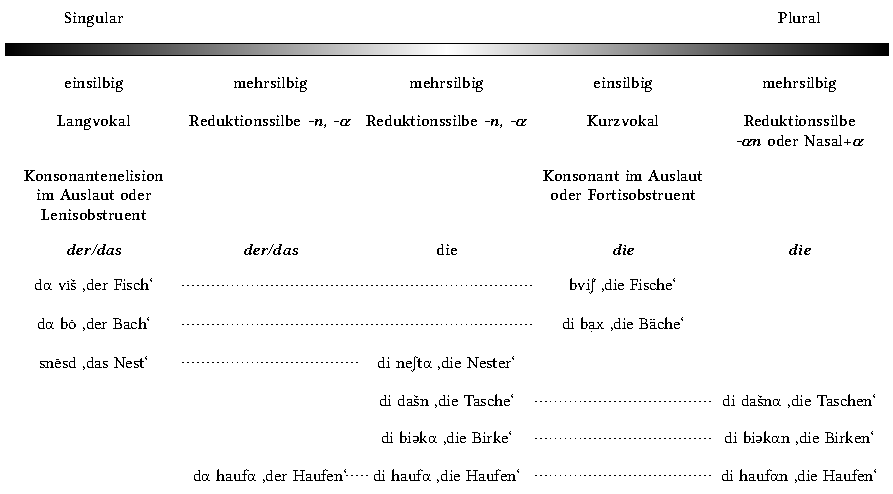
\includegraphics[width=\textwidth]{figures/fig10.2.pdf}
\caption{\label{fig:10.2}Kontinuum von Singular- und Plural-Schemata im Bair. mit Beispielen}
\label{fig:20}
\end{figure}

\citegen{Köpcke1993} Grundidee ist,\largerpage{} dass die schemabasierte Verarbeitung der Numerusinformation über probabilistische perzeptuelle Hinweisreize erfolgt. Übertragen auf die Formenbildung des Bair. heißt dies, dass wenig saliente und valide Cues wie Kontraste der Vokalquantität und des Konsonantismus in Kombination mit höher salienten und validen Cues (etwa dem Definitartikel) auftreten und ein Schema als Ganzes in Richtung der Singular- oder Pluralfunktion weist. Wenn also beispielsweise Lenis-Fortis-Kontraste, wie in \sectref{sec:7.1.2.3.1} festgestellt wurde, weniger binäre Merkmale sind, sondern innerhalb eines phonetischen Spektrums auftreten, so helfen die anderen Hinweisreize Vokalquantität und/oder Definitartikel die Wirkungsrichtung der Hinweisreize zu vereindeutigen. Dass der Hinweisreiz Vokalquantität (im Bair. in Kombination mit Lenis-Fortis-Kontrast) tatsächlich ein Schema konstituiert, kann an analogen Quantitätskontrasten bei historischem Langvokal oder Diphthong (etwa \teuthoo{va42o4sd}{vạ̄ọsd} -- \teuthoo{va43i.Sd}{vặiͅʃd} ‚Faust‘ im nordbair. Groschlattengrün) gesehen werden. Und auch die rein phonologisch bedingte Spirantisierung von /b/ in additiven Pluralformen des Typs \teuthoo{gro2b}{ɡrōb} -- \teuthoo{gre2wA}{ɡrēwα} ‚Grab‘ ist ein Hinweisreiz, der in Kombination mit dem salienten, ikonischen Tiefschwa-Suffix in Richtung Pluralfunktion weist (in \sectref{sec:7.1.2.3.3} wurde dies -- in Anlehnung an \citealt{Ronneberger-Sibold1990} -- noch als semiotische Funktion, als Indizieren des folgenden Pluralsuffixes, gefasst).

\begin{sloppypar}
Damit ist an dieser Stelle auch die in \chapref{chap:7} eingeführte methodische Schwierigkeit gelöst, welche Alternationen rein phonologisch bedingt sind und welche als genuin morphologisch (d.\,h. als funktionalisiert und produktiv) klassifiziert werden können. Die Vorannahme, dass letztlich alle innerparadigmatischen Alternationen morphologische Information symbolisieren, erweist sich als kognitiv plausibel; vor dem Hintergrund einer schemabasierten Perzeption sind aus Sprachnutzerperspektive alle der hier dargestellten Merkmale mehr oder weniger signalstark. Wie signalstark die einzelnen Komponenten eines Schemas im Einzelnen sind und wie groß ihr jeweiliger Beitrag zur Signalstärke des Schemas als Ganzes ist, muss allerdings noch empirisch überprüft werden.
\end{sloppypar}

\subsection{Feminina mit \textit{n}{}-Erweiterung aus Perspektive des Schema-Modells}
\label{sec:10.3.2}
Im Laufe der Untersuchung und auch der Diskussion standen die Feminina mit Nasalsuffix im Singular (Typ \teuthoo{das\#n}{dašn} -- \teuthoo{das\#n}{dašn} ‚Tasche‘) immer wieder im Fokus. Zum einen konnte anhand dieser Klasse gezeigt werden, dass im Bair. Numerusambiguitäten zum Teil morphologisch gelöst werden, während im Ofr. -- so ist zu vermuten -- der Numerussynkretismus im syntaktischen oder se\-man\-tisch-prag\-ma\-ti\-schen Kontext oder durch kommunikative Strategien disambiguiert wird. Zum anderen ist eines der Ergebnisse des bisherigen \chapref{chap:10}, dass die synkretischen Feminina, die ja überhaupt erst durch morphologischen Ausgleich entstanden sind, auch eine Herausforderung für die Vorhersagen der morphologischen Theoriebildung darstellen. Wie also lassen sich die \textit{n}{}-erweiterten Feminina vor dem Hintergrund des Schema-Ansatzes analysieren?

\citet[90]{Köpcke1993} sieht einen Beleg für die Unabhängigkeit von Schemata (in Abgrenzung zum relationalen Faktor eines lexikalischen Partners) in der diachronen Entwicklung der Feminina der historischen \textit{n}{}-Deklination. Synkretische Paradigmen, die bei einem Teil dieser Feminina durch lautgesetzlichen Wandel entstanden waren (ahd. \textit{ketina} > mhd. \textit{ketene} > \textit{ketten} > nhd. \textit{Kette}), wurden abgebaut zugunsten des distinkten Singular-Schemas [die + \#\_\_\_e] und des distinkten Plural-Schemas [die + \#\_\_\_en] (vgl. \citealt[§51]{Paul1968}). Da Substantive mit den sogenannten Pseudosuffixen -\textit{en} (\textit{Haufen}) und -\textit{er} (\textit{Fenster}) relativ zentrale Strukturmerkmale von Plural-Schemata aufweisen (nämlich die Pluralsuffixe -\textit{er} und -\textit{en}), ist die Vorhersage des Schema-Modells, „daß Feminina, die auf die Pseudosuffixe \mbox{-\textit{er}} und -\textit{en} auslauten, bei denen also seitens des Sprecher/Hörers Verwirrungen zu pluralen Gestalten auftreten können, im Laufe der historischen Entwicklung abgebaut werden“ \citep[119]{Köpcke1993}.

\citet[120]{Köpcke1993} erwähnt zwar, dass im Bair. das Nasalsuffix der historischen \textit{n}{}-Deklination auch auf die Singularform der Feminina ausgedehnt wurde, doch sei das Nasalsuffix „konsequenterweise“ und „sehr schnell“ wieder abgebaut worden zugunsten der historischen Schwa-Reduktionssilbe. Dieser Befund entspricht allerdings nicht den Realitäten der rezenten oobd. Dialekte. Trotzdem kann die Entwicklung der Feminina mit \textit{n}{}-Erweiterung in den bair. Dialekten ausgesprochen gut mit dem Schema-Ansatz modelliert werden.\footnote{Ausgenommen werden hier jene Dialekte des südlichen Mittelbair. und des mittelbair.-südbair. Übergangsgebiets, die präferiert apokopierte Singularstammformen und distinkte (additive) Pluralformen aufweisen (siehe \sectref{sec:8.2.3}); hier müssen wiederum eigene, dialektspezifische Schemata und Prototypen angenommen werden.} Das Bair. hat zwar ein fem. Schema [die + \#\_\_\_en] im Singular erhalten, doch wurde die Numerusambiguität durch die Schaffung eines spezifischen, prototypischen Plural-Schemas beseitigt. (Prototypikalität wird hier in Abgrenzung zu anderen pluralischen Schemata angenommen, weil [di+ \#\_\_\_-αn] und [di+ \#\_\_\_-nα] salient, valide und ikonisch sind.) Insbesondere das Schema [di+ \#\_\_\_-αn] hat in Teilen des Bair. „Sogwirkung“ \citep[103]{Köpcke1993} entwickelt: Auch Maskulina mit Tiefschwa-Reduktionssilbe markieren -- nach \citet[153]{Rowley1997} fakultativ -- den Plural mit Nasalsuffix (vgl. \sectref{sec:8.3.3.1}). Dass sich hier ein produktives, formales Konditionierungsmuster im südlichen Nordbair. und im Übergangsgebiet zum Mittelbair. herausgebildet hat, kann durch die Prototypikalität des Plural-Schemas und die Signalstärke der Hinweisreize in Richtung der Pluralinformation hergeleitet werden.


\begin{figure}
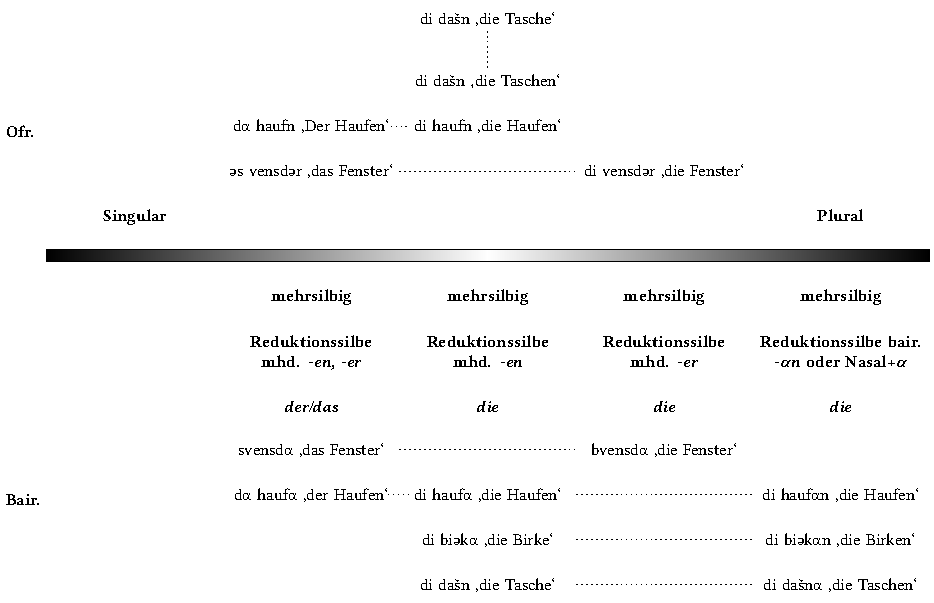
\includegraphics[width=\textwidth]{figures/fig10.3.pdf}
\caption{\label{fig:10.3} Schematisierung der relationalen Anordnung von Substantiven mit Reduktionssilbe mhd. \textit{-en}, \textit{-er} auf dem Singular-Plural-Kontinuum im Dialektvergleich}
\end{figure}

\begin{sloppypar}
Eine Herausforderung für die Voraussagen des Schema-Modells sind allerdings (wieder einmal) die Numerussynkretismen des Ofr. \figref{fig:10.3} bietet einen Vergleich der dialektalen Schemata von Substantiven mit Reduktionssilbe mhd. -\textit{en}, -\textit{er} auf dem Kontinuum von Singular- oder Plural-Schemata im Ofr. und Bair. Da die Entscheidung des Sprecher/Hörers zur Singularität oder Pluralität einer Substantivform durch die Faktoren absolute und relative Signalstärke erfolgt, kommt es im Ofr. beim fem. Schema [die + \#\_\_\_en] zu einem Unentschieden: Die absolute Signalstärke weist weder eindeutig in Richtung Singular noch Plural. Die relative Signalstärke kann allerdings auch nicht bestimmt werden, da es keinen lexikalischen Partner links oder rechts von \teuthoo{di}{di} \teuthoo{das\#n}{dašn} auf dem Kontinuum gibt; der Pl. \teuthoo{di}{di} \teuthoo{das\#n}{dašn} weist infolge des vollständigen Formensynkretismus von Definitartikel und Substantiv dieselben formalen Merkmale auf.
\end{sloppypar}

Dieses Unentschieden kann durch die bisher definierten morphologischen und morphosyntaktischen Hinweisreize nicht gelöst werden, da die Cues Reduktionssilbe (-\textit{n}) und Definitartikel (\textit{di}) für die schemabasierte Kategorisierung von morphologischen Informationen nicht eindeutig, nicht valide sind. Zur analytischen Kompetenz der Sprachnutzer gehört damit nicht nur die Assoziation und Repräsentation von Schemata zweiter Ordnung (d.\,h. von lexikalischen Partnern links oder rechts auf dem Singular-Plural-Kontinuum), sondern auch syntaktischer und semantisch-pragmatischer Kontext müssen bei der Verarbeitung der Numerusinformation analysiert werden. Die Frage ist nun, ob es in den Dialekten mit fem. Numerussynkretismen eine spezifisch fem. Verarbeitungsstrategie gibt, die bei Maskulina und Neutra nicht in dem Maße zum Einsatz kommt, da Einzelwort und NP (inklusive der Schemata zweiter Ordnung) verlässlichere Cues aufweisen. Interessant wäre es hier, die Entscheidungszeit bei der Verarbeitung der Numerusinformation zu messen (siehe etwa \citealt{KöpckeEtAl2021}) und zu vergleichen, wie sich die beiden Kompensations- und Kodierungsmodelle des UGs (auch unter Berücksichtigung von Genus) unterscheiden. Die Hypothese ist, dass die Numerusentscheidung im südlichen Nordbair. und Mittelbair. mit distinkten Pluralformen und validen Plural-Cues schneller erfolgt als im Ofr. und nördlichen Nordbair., da in diesem Kodierungsmodell für die Klassifikation als Singular- oder Pluralinformation mehr kontextuelle Information berücksichtigt werden muss. Dass der syntaktische und semantisch-pragmatische Kontext stärker in eine schemabasierte Modellierung von Sprachproduktion und -perzeption integriert werden muss, zeigen wiederum die fakultativen Plurale: Hier führt die sprecherseitige Analyse der Signalstärke der Hinweisreize zur Entscheidung, die Pluralität des Schemas durch zusätzliche morphologische Marker abzusichern. Damit ist Variabilität in der Kodierung der morphologischen Information in den Flexionssystemen mit fakultativer Pluralmarkierung Teil des Schemas und als Kodierungsstrategie zum Ausdruck des grammatischen Konzepts Plural auch Teil der mentalen Repräsentation.
